\chapter{template}

\section{Cross reference} \label{template_cross_reference}

The code snippet for list is given Section~\ref{template_list}.
The \texttt{~} makes sure three is a space between Section and the reference number but no new line split between them.



\section{Lists} \label{template_list}

\subsection{Bullet points}
\begin{itemize}
  \item Fish
  \item Animals
  \begin{itemize}
    \item Domesticated animals
    \begin{itemize}
      \item Cow
    \end{itemize}
  \end{itemize}
\end{itemize}
  
\subsection{Numbered list}

\begin{enumerate}
  \item Fish
  \item Animals
  \begin{enumerate}
    \item Domesticated animals
    \begin{enumerate}
      \item Cow
    \end{enumerate}
  \end{enumerate}
\end{enumerate}

\section{Code section}
\begin{lstlisting} [language=C,frame=single,caption=C code section,label=code1]
int main() {
  return 0;
}
\end{lstlisting}

\begin{lstlisting} [language=bash,frame=single,caption=bash code section,label=code1]
set logging file output.gdb
set logging on
\end{lstlisting}

\subsection{Figures}%
\label{sub:figures}

Figure~\ref{fig:Example} is an example figure.


\begin{figure}[h]
\caption{An example figure}
\centering
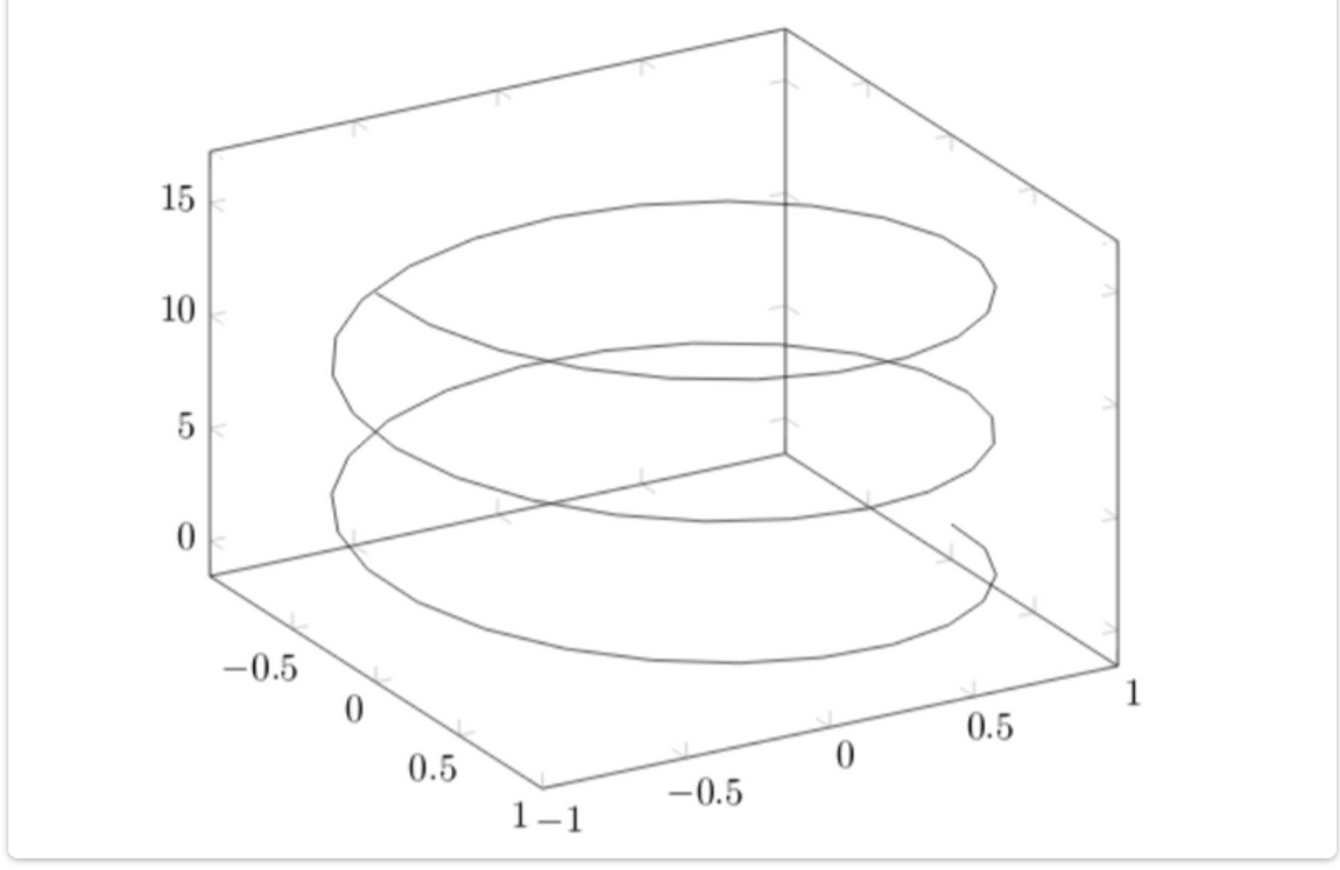
\includegraphics[width=0.5\textwidth]{./template/figure.pdf}
\label{fig:Example}
\end{figure}

\section{Reference}

\begin{enumerate}
  \item \href{https://www.google.com/}{google}
  \item \href{https://www.google.com/}{google}
\end{enumerate}
